\documentclass{BeamerTemplate}

\title{Chapitre 2 -- La théorie des probabilités (1\textsuperscript{re} partie)}
\subtitle{STT-1920 Méthodes statistiques}
\date{}

% ---------------------------------------------------------------------------
% Diagrammes de Venn (même style que STT-1900, Module 1)
% ---------------------------------------------------------------------------
\newcommand{\cadreVenn}{\draw (0,0) rectangle (4,3); \node at (3.7,2.7) {\scriptsize $\Omega$};}
\newcommand{\contourAB}{%
  \draw (1.5,1.5) circle (1); \node at (0.6,2.4) {$A$};
  \draw (2.5,1.5) circle (1); \node at (3.4,2.4) {$B$};}

% Styles des graphiques
\pgfplotsset{
  base/.style={
    tick label style={font=\scriptsize}, label style={font=\small},
    title style={font=\small\bfseries},
    yticklabel style={/pgf/number format/fixed, /pgf/number format/precision=2},
    scaled y ticks=false,
  },
  pmg/.style={base, xmin=42, xmax=63, xtick={45,50,55,60}, xlabel={$x$}},
}

\begin{document}

\begin{frame}[t]
  \titlepage
\end{frame}

%===============================================================================
\section{Probabilités et statistique}
%===============================================================================

\begin{frame}[t]{Où en sommes-nous?}
  Au chapitre 1, on a \alert{décrit} des données : histogramme, moyenne
  $\overline{x}$, écart-type $s$, quantiles, diagramme en boîte\ldots

  \medskip
  Pour tirer des conclusions sur une \alert{population} à partir d'un
  \alert{échantillon}, il faut un modèle du hasard.

  \bigskip
  \uncover<2->{
  \begin{Boite}{Probabilités}
    Outil mathématique formel servant à décrire et modéliser les comportements
    aléatoires.
  \end{Boite}
  On connaît les « paramètres » du phénomène et on décrit ce qu'on attend.

  \medskip
  \textbf{Exemple :} Une génisse a autant de chances d'avoir une femelle
  qu'un mâle. Quelle est la probabilité d'avoir au moins une femelle parmi ses
  trois premiers veaux?
  }
\end{frame}

\begin{frame}[t]{Probabilités vs statistique}
  \begin{Boite}{Statistique}
    Étude quantitative des attributs d'une « population » à partir
    d'observations.
  \end{Boite}
  On ne connaît pas les « paramètres » du phénomène : c'est ce qu'on tente
  d'estimer.

  \medskip
  \textbf{Exemple :} Sur 200 vêlages observés, 112 ont donné une femelle.
  Peut-on encore croire que les deux sexes sont équiprobables?

  \bigskip
  \uncover<2->{
  $\Rightarrow$ Le caractère \alert{aléatoire} de l'échantillonnage fait que
  la statistique repose sur la théorie des probabilités. C'est l'objet de ce
  chapitre.
  }
\end{frame}

%===============================================================================
\section[Expérience aléatoire]{2.1 Expérience aléatoire et événements}
%===============================================================================

\begin{frame}[t]{Expérience aléatoire}
  \begin{Boite}{Expérience aléatoire $\mathcal{E}$}
    Expérience dont le résultat dépend du hasard, ne pouvant être prédit avec
    certitude.
  \end{Boite}

  \begin{Boite}{Espace échantillonnal $\Omega$ (ou ensemble fondamental)}
    Ensemble de tous les résultats possibles de l'expérience $\mathcal{E}$.
    Le nombre d'éléments de $\Omega$ est appelé le \emph{cardinal} de $\Omega$.
  \end{Boite}

  \begin{itemize}
    \item \alert{$\Omega$ discret} : si $\Omega$ est fini ou dénombrable
      (ex. : la liste des entiers)
    \item \alert{$\Omega$ continu} : si $\Omega$ est non dénombrable
      (ex. : un intervalle de valeurs sur la droite réelle)
  \end{itemize}
\end{frame}

\begin{frame}[t]{Exemple 1 : quel est l'espace échantillonnal?}
  \begin{itemize}\itemsep 7mm
    \item $\mathcal{E}_1$ : on note le sexe des trois premiers veaux d'une génisse.
      \uncover<2->{\alert{$\Rightarrow \Omega_1 = \{FFF, FFM, FMF, MFF, FMM, MFM, MMF, MMM\}$}}
    \item $\mathcal{E}_2$ : on compte le nombre de lésions foliaires sur une
      parcelle de gazon de 1\,m sur 2\,m.
      \uncover<3->{\alert{$\Rightarrow \Omega_2 = \{0, 1, 2, \ldots\}$}}
    \item $\mathcal{E}_3$ : on mesure les précipitations (en mm) reçues à
      Québec en juillet.
      \uncover<4->{\alert{$\Rightarrow \Omega_3 = [0, \infty)$}}
  \end{itemize}

  \bigskip
  \uncover<5->{Lesquels de ces espaces sont discrets? continus?}
\end{frame}

\begin{frame}[t]{Événement}
  \begin{Boite}{Événement}
    Sous-ensemble de l'espace échantillonnal $\Omega$. On utilise une lettre
    majuscule pour l'identifier.
  \end{Boite}

  \medskip
  \uncover<2->{
  Retour aux expériences de l'exemple 1 :
  \begin{itemize}\itemsep 4mm
    \item $\mathcal{E}_1$ : $A$ = « au moins une femelle »
      $= \{FFF, FFM, FMF, MFF, FMM, MFM, MMF\}$
    \item $\mathcal{E}_2$ : $C$ = « moins de 10 lésions » $= \{0, 1, \ldots, 9\}$
    \item $\mathcal{E}_3$ : $D$ = « plus de 150\,mm de pluie » $= (150, \infty)$
  \end{itemize}
  }
\end{frame}

\begin{frame}[t]{Exemple 2 : une espèce envahissante}
  \begin{columns}[T]
    \column{0.52\textwidth}
      L'hydrocharis grenouillère est une plante aquatique flottante envahissante.

      \medskip
      $\mathcal{E}$ : à plusieurs points d'un lac,
      \begin{itemize}\small
        \item on note la présence de l'hydrocharis;
        \item on note la présence d'un autre macrophyte flottant;
        \item on mesure la profondeur du lac.
      \end{itemize}

      \medskip
      Espace échantillonnal?
      \vspace{1.2cm}

      Quelques événements?
    \column{0.45\textwidth}
      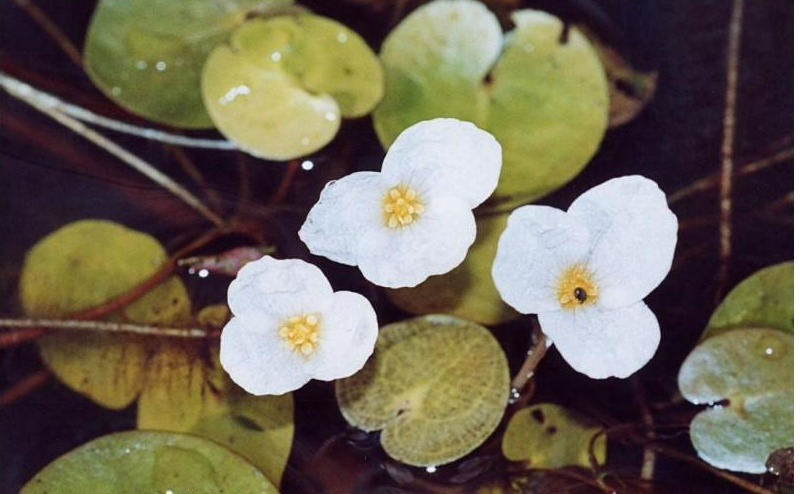
\includegraphics[width=\linewidth]{images/hydrocharis.jpg}

      {\tiny\itshape Christian Fischer, CC BY-SA 3.0,
      \url{https://commons.wikimedia.org/w/index.php?curid=1042515}}
  \end{columns}
\end{frame}

\begin{frame}{Rappel des opérations sur les ensembles}
  \begin{columns}
    \column{0.5\textwidth}
      \textbf{1) Complément de $A$ : $A^c$}
      \vspace{0.2cm}

      \begin{tikzpicture}[scale=0.8]
        \fill[gray!30] (0,0) rectangle (4,3);
        \fill[Fond] (1.5,1.5) circle (1);
        \cadreVenn
        \draw (1.5,1.5) circle (1); \node at (0.6,2.4) {$A$};
      \end{tikzpicture}

      \vspace{0.3cm}
      \textbf{3) Intersection de $A$ et $B$ : $A \cap B$}
      \vspace{0.2cm}

      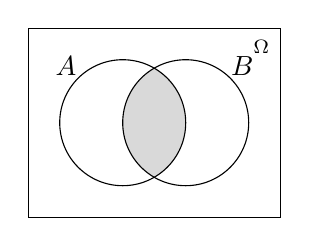
\begin{tikzpicture}[scale=0.8]
        \begin{scope}\clip (1.5,1.5) circle (1); \fill[gray!30] (2.5,1.5) circle (1);\end{scope}
        \cadreVenn \contourAB
      \end{tikzpicture}
    \column{0.5\textwidth}
      \textbf{2) Inclusion de $B$ dans $A$ : $B \subset A$}
      \vspace{0.2cm}

      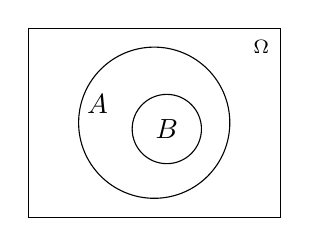
\begin{tikzpicture}[scale=0.8]
        \cadreVenn
        \draw (2,1.5) circle (1.2); \node at (1.1,1.8) {$A$};
        \draw (2.2,1.4) circle (0.55); \node at (2.2,1.4) {$B$};
      \end{tikzpicture}

      \vspace{0.3cm}
      \textbf{4) Union de $A$ et $B$ : $A \cup B$}
      \vspace{0.2cm}

      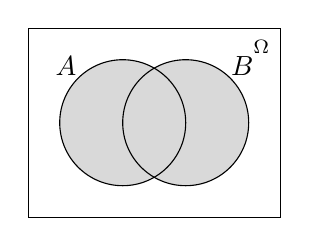
\begin{tikzpicture}[scale=0.8]
        \fill[gray!30] (1.5,1.5) circle (1); \fill[gray!30] (2.5,1.5) circle (1);
        \cadreVenn \contourAB
      \end{tikzpicture}
  \end{columns}
\end{frame}

\begin{frame}[t]{Événements mutuellement exclusifs}
  \begin{Boite}{Événements mutuellement exclusifs (ou disjoints)}
    Des événements sont \alert{mutuellement exclusifs} si toutes leurs
    intersections possibles sont vides, c'est-à-dire lorsqu'\textbf{au plus un}
    de ces événements peut se produire à la fois.
  \end{Boite}

  \medskip
  \uncover<2->{
  En d'autres termes, $A$, $B$ et $C$ sont mutuellement exclusifs si
  \[
    A \cap B = \varnothing, \quad A \cap C = \varnothing, \quad
    B \cap C = \varnothing \quad \text{et} \quad A \cap B \cap C = \varnothing.
  \]
  }
\end{frame}

\begin{frame}[plain,t]
  \centerline{\LARGE\bfseries\alert{QUIZ !}}

  \medskip
  Les événements suivants sont-ils mutuellement exclusifs?
  \begin{itemize}\itemsep 1.4cm
    \item $\mathcal{E}_1$ : sexe des trois premiers veaux.\\
      $A$ = « au moins une femelle », $B$ = « trois mâles » et
      $C$ = « exactement deux femelles ».
    \item<2-> $\mathcal{E}_3$ : précipitations en juillet.\\
      $A$ = « plus de 150\,mm », $B$ = « moins de 175\,mm » et
      $C$ = « entre 200 et 300\,mm ».
  \end{itemize}
\end{frame}

\begin{frame}[t]{Interprétation d'une probabilité}
  La probabilité d'un événement $A$, notée $P(A)$, est un nombre entre 0 et 1
  qui mesure ses chances de survenir.

  \medskip
  \uncover<2->{
  \begin{Boite}{Fréquence relative d'un événement}
    On répète $m$ fois une expérience $\mathcal{E}$ et on note $m_A$ le nombre
    de fois où l'événement $A$ se produit. Alors $f_A = m_A / m$ est la
    \alert{fréquence relative} de $A$.
  \end{Boite}
  }
  \uncover<3->{
  Intuitivement, $P(A)$ est la fréquence relative de $A$ lorsqu'on répète
  l'expérience un très grand nombre de fois :
  \[ P(A) = \lim_{m \to \infty} \frac{m_A}{m}. \]
  }
\end{frame}

\begin{frame}[t]{La fréquence relative se stabilise}
  On simule 1000 vêlages et on suit la proportion de femelles obtenues.

  \centering
  \begin{tikzpicture}
    \begin{axis}[base, width=0.85\textwidth, height=0.62\textheight,
        xlabel={Nombre de vêlages $m$}, ylabel={Fréquence relative $f_A$},
        ymin=0, ymax=1, xmin=0, xmax=1000]
      \addplot[thick, Accent] coordinates {(1,1.0000) (2,0.5000) (3,0.6667) (4,0.7500) (5,0.6000) (6,0.5000) (7,0.4286) (8,0.3750) (9,0.4444) (10,0.5000) (11,0.5455) (12,0.5833) (13,0.6154) (14,0.5714) (15,0.6000) (16,0.6250) (17,0.5882) (18,0.5556) (19,0.5789) (20,0.5500) (30,0.6333) (40,0.6500) (50,0.5800) (60,0.5667) (70,0.5571) (80,0.5250) (90,0.5222) (100,0.5300) (110,0.5182) (120,0.5083) (130,0.5154) (140,0.5286) (150,0.5267) (160,0.5250) (170,0.5118) (180,0.5111) (190,0.5211) (200,0.5150) (210,0.5095) (220,0.5045) (230,0.5043) (240,0.4917) (250,0.4800) (260,0.4731) (270,0.4778) (280,0.4679) (290,0.4655) (300,0.4733) (310,0.4677) (320,0.4688) (330,0.4667) (340,0.4735) (350,0.4743) (360,0.4694) (370,0.4730) (380,0.4658) (390,0.4641) (400,0.4625) (410,0.4659) (420,0.4643) (430,0.4628) (440,0.4614) (450,0.4622) (460,0.4543) (470,0.4553) (480,0.4562) (490,0.4612) (500,0.4560) (510,0.4549) (520,0.4596) (530,0.4604) (540,0.4648) (550,0.4636) (560,0.4643) (570,0.4632) (580,0.4586) (590,0.4576) (600,0.4583) (610,0.4623) (620,0.4597) (630,0.4619) (640,0.4641) (650,0.4615) (660,0.4621) (670,0.4627) (680,0.4618) (690,0.4652) (700,0.4643) (710,0.4634) (720,0.4597) (730,0.4575) (740,0.4554) (750,0.4547) (760,0.4566) (770,0.4558) (780,0.4551) (790,0.4532) (800,0.4537) (810,0.4543) (820,0.4549) (830,0.4590) (840,0.4560) (850,0.4600) (860,0.4616) (870,0.4632) (880,0.4648) (890,0.4640) (900,0.4622) (910,0.4593) (920,0.4630) (930,0.4613) (940,0.4596) (950,0.4589) (960,0.4562) (970,0.4557) (980,0.4592) (990,0.4596) (1000,0.4570)};
      \addplot[dashed, black, domain=0:1000] {0.5};
      \node[anchor=south east, font=\scriptsize] at (axis cs:990,0.52) {$P(A) = 0.5$};
    \end{axis}
  \end{tikzpicture}
\end{frame}

%===============================================================================
\section[Propriétés]{2.2 Propriétés des probabilités}
%===============================================================================

\begin{frame}[t]
  \begin{defn}
    Soit une expérience aléatoire $\mathcal{E}$ et son espace échantillonnal
    $\Omega$. Si un événement $A$ est défini dans $\Omega$, alors la
    \alert{probabilité de $A$, notée $P(A)$}, est un nombre réel respectant les
    axiomes\footnote{Point de départ d'un raisonnement considéré comme non
    démontrable, évident. (Larousse)} suivants :
    \begin{enumerate}
      \item $0 \le P(A) \le 1$
      \item $P(\Omega) = 1$
      \item Pour toute suite d'événements \alert{mutuellement exclusifs}
        $A_1, A_2, \ldots, A_k$ définis dans $\Omega$, on a
        \[ P(A_1 \cup A_2 \cup \cdots \cup A_k) = P(A_1) + P(A_2) + \cdots + P(A_k). \]
      \item L'axiome 3 reste vrai quand $k \to \infty$.
    \end{enumerate}
  \end{defn}
  Ce sont les \emph{axiomes de Kolmogorov} (p.~29 des notes).
\end{frame}

\begin{frame}[t]{Spécification des probabilités}
  Comment peut-on déterminer des probabilités?

  \medskip
  \begin{itemize}\itemsep 8mm
    \item<1-> estimations basées sur des observations\\
      {\small\color{gray} (ex. : 85\,\% des grains d'un lot d'avoine germent)}
    \item<2-> analyse des conditions expérimentales\\
      {\small\color{gray} (ex. : un dé régulier, une pièce équilibrée)}
    \item<3-> modèles probabilistes et/ou hypothèses\\
      {\small\color{gray} (ex. : chaque vêlage donne une femelle avec probabilité 1/2,
      indépendamment des autres)}
  \end{itemize}
\end{frame}

\begin{frame}[t]{Le cas équiprobable}
  \begin{prp}
    Si $\Omega$ est un ensemble fini et si tous les résultats possibles ont la
    même probabilité, alors pour tout événement $A$,
    \[ P(A) = \frac{\operatorname{cardinal}(A)}{\operatorname{cardinal}(\Omega)}. \]
  \end{prp}

  \uncover<2->{
  \textbf{Retour à l'exemple 1 :} si les deux sexes sont équiprobables à
  chaque vêlage, les 8 résultats de $\Omega_1$ sont équiprobables. Donc
  \[ P(\text{« exactement deux femelles »}) = \frac{\operatorname{cardinal}\{FFM, FMF, MFF\}}{8} = \frac{3}{8}. \]
  }
\end{frame}

\begin{frame}[t]{Résultats découlant des axiomes}
  Les résultats qui suivent sont des conséquences des axiomes.

  \begin{itemize}\itemsep 3mm
    \item<1-> \textbf{Ensemble vide :} $P(\varnothing) = 0$

      {\color{gray}[$\Omega$ et $\varnothing$ sont mutuellement exclusifs,
      $\Omega \cup \varnothing = \Omega$ et $P(\Omega) = 1$\ldots]}
    \item<2-> \textbf{Complément :} $P(A) = 1 - P(A^c)$

      {\color{gray}[$A$ et $A^c$ sont mutuellement exclusifs et
      $\Omega = A \cup A^c$\ldots]}
    \item<3-> \textbf{Formule de Poincaré :}
      $P(A \cup B) = P(A) + P(B) - P(A \cap B)$
    \item<4-> et pour trois événements :
      \[
        \begin{array}{lll}
          P(A \cup B \cup C) &=& P(A) + P(B) + P(C) \\
          && - P(A \cap B) - P(A \cap C) - P(B \cap C) \\
          && + P(A \cap B \cap C)
        \end{array}
      \]
  \end{itemize}
\end{frame}

\begin{frame}[t]{Formule de Poincaré : pourquoi soustraire $P(A \cap B)$?}
  \centering
  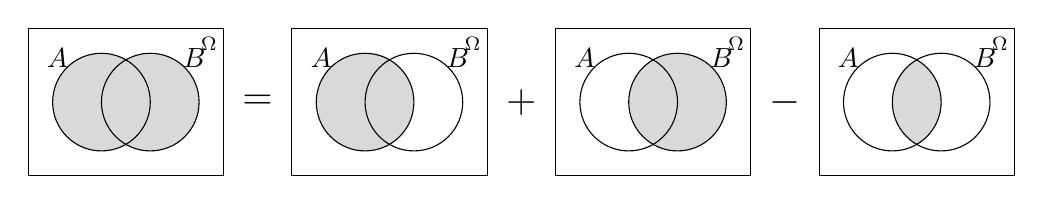
\begin{tikzpicture}[scale=0.62]
    \begin{scope}
      \fill[gray!30] (1.5,1.5) circle (1); \fill[gray!30] (2.5,1.5) circle (1); \cadreVenn \contourAB
    \end{scope}
    \node at (4.7,1.5) {\Large $=$};
    \begin{scope}[xshift=5.4cm]
      \fill[gray!30] (1.5,1.5) circle (1); \cadreVenn \contourAB
    \end{scope}
    \node at (10.1,1.5) {\Large $+$};
    \begin{scope}[xshift=10.8cm]
      \fill[gray!30] (2.5,1.5) circle (1); \cadreVenn \contourAB
    \end{scope}
    \node at (15.5,1.5) {\Large $-$};
    \begin{scope}[xshift=16.2cm]
      \begin{scope}\clip (1.5,1.5) circle (1); \fill[gray!30] (2.5,1.5) circle (1);\end{scope}
      \cadreVenn \contourAB
    \end{scope}
  \end{tikzpicture}

  \bigskip
  \raggedright
  En additionnant $P(A)$ et $P(B)$, la zone $A \cap B$ est comptée
  \alert{deux fois}.
\end{frame}

\begin{frame}[t]{Résultats utiles}
  Ces deux résultats (lois de De Morgan) sont souvent utiles :
  \begin{align*}
    P\big((A \cap B)^c\big) &= P(A^c \cup B^c) \\
    P\big((A \cup B)^c\big) &= P(A^c \cap B^c)
  \end{align*}

  \uncover<2->{
  \textbf{Exemple :} « ni l'espèce $A$ ni l'espèce $B$ n'est présente »
  $= A^c \cap B^c = (A \cup B)^c$.
  }
\end{frame}

\begin{frame}[t]{Exemple 1 (suite)}
  En supposant qu'une génisse a autant de chances d'accoucher d'une femelle
  que d'un mâle à chaque gestation, quelle est la probabilité qu'elle ait
  \alert{au moins une femelle} parmi ses 3 premiers petits?

  \vspace{3cm}
  \uncover<2->{{\small\color{gray} Indice : quel est le complément de
  « au moins une femelle »?}}
\end{frame}

\begin{frame}[t]{Exemple 2 (suite)}
  \small
  Les photographies aériennes du lac montrent que l'hydrocharis grenouillère
  (espèce $A$) est présente dans 15\,\% de la superficie du lac. Il n'y a
  qu'une autre espèce de macrophyte flottant (espèce $B$), présente dans
  25\,\% de la superficie. Au total, 35\,\% de la superficie du lac est
  occupée par les macrophytes flottants.

  \begin{enumerate}[a)]\itemsep 1.1cm
    \item Quelle portion du lac est une zone d'eau libre, inoccupée par les
      macrophytes?
    \item Si on choisit un site d'échantillonnage au hasard, quelle est la
      probabilité de tomber sur une zone bispécifique (les deux espèces
      présentes)?
  \end{enumerate}
\end{frame}

\begin{frame}[t]{Exemple 2 : piste de solution}
  Remplir toutes les zones mutuellement exclusives d'un diagramme de Venn.\\
  $A$ = « l'hydrocharis est présente », $B$ = « l'autre macrophyte est présent ».

  \bigskip
  \centering
  \begin{tikzpicture}[scale=1.25]
    \cadreVenn \contourAB
    \node<2->[font=\footnotesize, text=burntorange] at (1.0,1.5) {0.10};
    \node<2->[font=\footnotesize, text=burntorange] at (2.0,1.5) {0.05};
    \node<2->[font=\footnotesize, text=burntorange] at (3.0,1.5) {0.20};
    \node<2->[font=\footnotesize, text=burntorange] at (0.45,0.3) {0.65};
  \end{tikzpicture}
\end{frame}

%===============================================================================
\section[Analyse combinatoire]{2.3 Notions d'analyse combinatoire}
%===============================================================================

\begin{frame}[t]{Pourquoi compter?}
  Dans le \alert{cas équiprobable},
  $P(A) = \operatorname{cardinal}(A) / \operatorname{cardinal}(\Omega)$ :
  il suffit de \alert{compter}.

  \medskip
  Avec 3 veaux, on peut énumérer les 8 résultats à la main. Mais\ldots
  \begin{itemize}\itemsep 2mm
    \item avec 10 veaux, combien de séquences $F$/$M$ possibles?
    \item combien d'échantillons différents de 5 semences peut-on prélever
      dans un lot de 20?
  \end{itemize}

  \medskip
  \uncover<2->{
  $\Rightarrow$ L'\alert{analyse combinatoire} regroupe les techniques de
  dénombrement utiles pour ces calculs (section 2.3 des notes). Trois outils
  suffisent pour ce cours : le principe de multiplication, les
  \alert{permutations} et les \alert{combinaisons}.
  }
\end{frame}

\begin{frame}[t]{Principe fondamental du dénombrement}
  \begin{Boite}{Principe fondamental du dénombrement}
    Si une procédure comporte $k$ étapes successives, avec $n_1$ façons de
    réaliser la 1\textsuperscript{re} étape, puis $n_2$ façons de réaliser la
    2\textsuperscript{e} (peu importe le choix fait à la 1\textsuperscript{re}),
    \ldots, puis $n_k$ façons de réaliser la $k$\textsuperscript{e}, alors il y
    a en tout
    \[ n_1 \times n_2 \times \cdots \times n_k \]
    façons de réaliser la procédure.
  \end{Boite}

  \begin{itemize}\itemsep 1mm
    \item<2-> Essai agronomique : 3 variétés de blé $\times$ 4 doses d'engrais
      $\times$ 2 régimes d'irrigation $= 24$ traitements.
    \item<3-> Exemple 1 : chaque veau est $F$ ou $M$, donc
      $2 \times 2 \times 2 = 2^3 = 8$ résultats. Avec 10 veaux :
      $2^{10} = 1024$ résultats.
  \end{itemize}
\end{frame}

\begin{frame}[t]{Permutations}
  Une \alert{permutation} est un arrangement \alert{ordonné} d'objets :
  l'ordre compte.

  \begin{Boite}{Nombre de permutations}
    \begin{itemize}
      \item de $n$ objets : $n! = n \times (n-1) \times \cdots \times 2 \times 1$
        \ (« $n$ factoriel »; $0! = 1$);
      \item de $k$ objets choisis parmi $n$ :
        $\displaystyle P_{n,k} = n \times (n-1) \times \cdots \times (n-k+1)
        = \frac{n!}{(n-k)!}$.
    \end{itemize}
  \end{Boite}

  \uncover<2->{
  \begin{itemize}\itemsep 1mm
    \item Ordre de passage de 5 échantillons sanguins dans un analyseur :
      $5! = 120$ ordres possibles.
    \item On attribue 3 traitements \emph{différents} ($T_1$, $T_2$, $T_3$) à
      3 des 8 parcelles d'un champ (une parcelle par traitement) :
      $P_{8,3} = 8 \times 7 \times 6 = 336$ façons.
  \end{itemize}
  }
\end{frame}

\begin{frame}[t]{Combinaisons}
  Une \alert{combinaison} de $k$ objets parmi $n$ est un sous-ensemble de $k$
  objets : l'ordre \alert{ne compte pas}.

  \begin{Boite}{Nombre de combinaisons (coefficient binomial)}
    \[ \binom{n}{k} = C_{n,k} = \frac{n!}{k!\,(n-k)!} = \frac{P_{n,k}}{k!} \]
  \end{Boite}
  {\small Chaque combinaison de $k$ objets correspond à $k!$ permutations :
  on divise donc par $k!$.}

  \uncover<2->{
  \begin{itemize}\itemsep 1mm
    \item On choisit 3 des 8 parcelles pour recevoir \emph{le même} engrais :
      $\binom{8}{3} = 56$ façons (et non 336).
    \item Exemple 1 : séquences de 3 veaux avec exactement 2 femelles
      $= \binom{3}{2} = 3$ (on choisit la position des 2 $F$).
  \end{itemize}
  }
\end{frame}

\begin{frame}[t]{Exemple 3 : un lot de semences}
  Un lot de 20 semences contient 4 semences infectées par un champignon
  pathogène. On en prélève 5 au hasard (sans remise) pour les analyser.

  \begin{enumerate}[a)]\itemsep 5mm
    \item Combien d'échantillons de 5 semences différents peut-on prélever?

      \uncover<2->{\alert{$\binom{20}{5} = 15\,504$ échantillons, tous
      équiprobables.}}
    \item Quelle est la probabilité qu'aucune semence infectée ne soit
      prélevée?

      \uncover<3->{\alert{Il faut choisir les 5 semences parmi les 16 saines :
      $\dfrac{\binom{16}{5}}{\binom{20}{5}} = \dfrac{4\,368}{15\,504}
      \approx 0.282$.}}
    \item Quelle est la probabilité que l'échantillon contienne exactement une
      semence infectée?

      \uncover<4->{{\small\color{gray} Indice : choisir 1 infectée parmi 4
      \emph{et} 4 saines parmi 16.}}
  \end{enumerate}

  \medskip
  \uncover<2->{{\small\color{gray} Dans R : \texttt{factorial(5)} donne
  $5!$ et \texttt{choose(20, 5)} donne $\binom{20}{5}$.}}
\end{frame}

\begin{frame}[plain,t]
  \centerline{\LARGE\bfseries\alert{QUIZ !}}

  \medskip
  Permutation ou combinaison? Combien de possibilités?
  \begin{itemize}\itemsep 1.0cm
    \item On forme un comité de protection des animaux de 4 membres parmi 9
      chercheurs.
    \item On dépose 6 échantillons d'ADN dans les 6 puits d'un gel
      d'électrophorèse. Combien d'ordres de dépôt?
    \item Un généticien choisit 2 lignées parmi 7 pour un croisement : l'une
      servira de mère, l'autre de père.
    \item<2-> Retour à l'exemple 1 : quelle est la probabilité qu'une génisse
      ait exactement 2 femelles parmi ses 10 premiers veaux?
  \end{itemize}
\end{frame}

%===============================================================================
\section[Probabilité conditionnelle]{2.4 Probabilité conditionnelle et indépendance}
%===============================================================================

\begin{frame}[t]{Une information partielle change les probabilités}
  Retour à l'exemple 2 : $P(A) = 0.15$, $P(B) = 0.25$ et
  $P(A \cap B) = 0.05$.

  \medskip
  On choisit un site au hasard et on nous apprend que \alert{l'espèce $B$ y
  est présente}. Quelle est maintenant la probabilité d'y trouver
  l'hydrocharis?

  \medskip
  \begin{columns}[c]
    \column{0.42\textwidth}
      \centering
      \begin{tikzpicture}[scale=0.9]
        \fill<2->[Dominante!40] (2.5,1.5) circle (1);
        \begin{scope}\clip (1.5,1.5) circle (1);
          \fill<2->[Accent!80] (2.5,1.5) circle (1);\end{scope}
        \cadreVenn \contourAB
        \node<2->[font=\scriptsize] at (2.0,1.5) {0.05};
        \node<2->[font=\scriptsize] at (3.0,1.5) {0.20};
      \end{tikzpicture}
    \column{0.55\textwidth}
      \uncover<2->{%
      On sait qu'on est dans $B$ : \alert{$B$ devient le nouvel espace
      échantillonnal}. Quelle fraction de $B$ est aussi dans $A$?
      \[ \frac{P(A \cap B)}{P(B)} = \frac{0.05}{0.25} = 0.20. \]
      }
      \uncover<3->{%
      L'information « $B$ est présente » fait passer la probabilité de $A$ de
      0.15 à 0.20.
      }
  \end{columns}
\end{frame}

\begin{frame}[t]{Probabilité conditionnelle}
  \begin{defn}
    Soit $A$ et $B$ deux événements avec $P(B) > 0$. La \alert{probabilité
    conditionnelle de $A$ sachant $B$} est
    \[ P(A \mid B) = \frac{P(A \cap B)}{P(B)}. \]
  \end{defn}

  \uncover<2->{
  $P(\,\cdot \mid B)$ respecte tous les axiomes et leurs conséquences :
  $0 \le P(A \mid B) \le 1$, $P(B \mid B) = 1$,
  $P(A^c \mid B) = 1 - P(A \mid B)$, etc.
  }

  \uncover<3->{
  \begin{Boite}{Règle de multiplication (on isole l'intersection)}
    \[ P(A \cap B) = P(A \mid B)\,P(B) = P(B \mid A)\,P(A) \]
  \end{Boite}
  Très utile quand l'expérience se déroule \alert{en étapes successives}.
  }
\end{frame}

\begin{frame}[t]{Attention : $P(A \mid B) \neq P(B \mid A)$ !}
  Retour à l'exemple 2 :
  \[
    P(A \mid B) = \frac{0.05}{0.25} = 0.20
    \qquad \text{mais} \qquad
    P(B \mid A) = \frac{0.05}{0.15} \approx 0.33.
  \]
  \begin{itemize}
    \item 20\,\% des sites occupés par l'espèce $B$ contiennent aussi
      l'hydrocharis;
    \item 33\,\% des sites occupés par l'hydrocharis contiennent aussi
      l'espèce $B$.
  \end{itemize}

  \medskip
  \uncover<2->{
  \textbf{Autre exemple :} presque toutes les personnes atteintes de la
  rougeole font de la fièvre : $P(\text{fièvre} \mid \text{rougeole})
  \approx 1$. Mais parmi les personnes qui font de la fièvre, très peu ont la
  rougeole : $P(\text{rougeole} \mid \text{fièvre})$ est très petite.
  }

  \medskip
  \uncover<3->{
  Confondre les deux est une erreur \alert{très fréquente}. On la retrouvera
  avec les tests diagnostiques (plus loin) et avec les tests d'hypothèses.
  }
\end{frame}

\begin{frame}[t]{Exemple 3 (suite) : tirages successifs}
  Lot de 20 semences, dont 4 infectées. On tire 2 semences \alert{l'une après
  l'autre}, sans remise. Soit $I_1$ = « la 1\textsuperscript{re} est infectée »
  et $I_2$ = « la 2\textsuperscript{e} est infectée ».

  \begin{enumerate}[a)]\itemsep 7mm
    \item Que vaut $P(I_1)$?
      \uncover<2->{\alert{$4/20 = 0.2$}}
    \item Que vaut $P(I_2 \mid I_1)$?
      \uncover<3->{\alert{Il reste 19 semences, dont 3 infectées :
      $3/19$.}}
    \item Quelle est la probabilité que les deux semences soient infectées?

      \uncover<4->{\alert{$P(I_1 \cap I_2) = P(I_1)\,P(I_2 \mid I_1)
      = \dfrac{4}{20} \times \dfrac{3}{19} = \dfrac{12}{380} \approx 0.0316$.}}
  \end{enumerate}

  \medskip
  \uncover<5->{{\small\color{gray} Vérification par dénombrement :
  $\binom{4}{2} \big/ \binom{20}{2} = 6/190 \approx 0.0316$.}}
\end{frame}

\begin{frame}[plain,t]
  \centerline{\LARGE\bfseries\alert{QUIZ !}}

  \medskip
  Supposons $P(B) > 0$. Que vaut $P(A \mid B)$\ldots
  {\small\color{gray} (faites un diagramme de Venn!)}
  \begin{itemize}\itemsep 1.2cm
    \item si $B \subset A$?
    \item si $A \subset B$?
    \item si $A$ et $B$ sont mutuellement exclusifs?
  \end{itemize}
\end{frame}

\subsection{Indépendance}

\begin{frame}[t]{Indépendance de deux événements}
  Je note le sexe d'un veau, puis je lance une pièce de monnaie. Soit les
  événements
  \begin{itemize}
    \item $A$ = « le veau est une femelle »;
    \item $B$ = « la pièce indique face ».
  \end{itemize}

  \medskip
  Le fait que $A$ se réalise ou non n'a aucun impact sur la probabilité de $B$!

  \medskip
  On dira alors que $A$ et $B$ sont \alert{indépendants}.

  \medskip
  \uncover<2->{
  \begin{Boite}{Indépendance de deux événements (section 2.4)}
    Deux événements $A$ et $B$ sont \alert{indépendants} si et seulement si
    \[ P(A \cap B) = P(A) \cdot P(B). \]
  \end{Boite}
  }
\end{frame}

\begin{frame}[t]{Indépendance et probabilité conditionnelle}
  Si $P(B) > 0$, la règle de multiplication donne
  $P(A \cap B) = P(A \mid B)\,P(B)$. Donc
  \begin{Boite}{Reformulation}
    $A$ et $B$ sont indépendants $\iff$ $P(A \mid B) = P(A)$.
  \end{Boite}
  Savoir que $B$ s'est réalisé \alert{ne change pas} la probabilité de $A$.

  \medskip
  \uncover<2->{
  \textbf{Plus de deux événements :} $A$, $B$ et $C$ sont
  \alert{(mutuellement) indépendants} si
  \[
    P(A \cap B) = P(A)\,P(B), \quad P(A \cap C) = P(A)\,P(C), \quad
    P(B \cap C) = P(B)\,P(C)
  \]
  \[ \text{et} \quad P(A \cap B \cap C) = P(A)\,P(B)\,P(C). \]
  }
  \uncover<3->{%
  \textbf{Exemple 1 :} si les vêlages sont indépendants et que
  $P(F) = 1/2$ à chaque vêlage, alors
  $P(MMM) = \frac12 \cdot \frac12 \cdot \frac12 = \frac18$. C'est ce qui
  justifie que les 8 résultats de $\Omega_1$ sont équiprobables.
  }
\end{frame}

\begin{frame}[plain,t]
  \centerline{\LARGE\bfseries\alert{QUIZ !}}

  \medskip
  Retour à l'exemple 2 : $P(A) = 0.15$, $P(B) = 0.25$, $P(A \cup B) = 0.35$.

  \begin{itemize}\itemsep 1.5cm
    \item La présence de l'espèce $A$ est-elle indépendante de celle de
      l'espèce $B$?
    \item S'agit-il d'événements mutuellement exclusifs?
    \item<2-> Deux événements mutuellement exclusifs, chacun de probabilité
      positive, peuvent-ils être indépendants?
  \end{itemize}
\end{frame}

\subsection{Probabilités totales et théorème de Bayes}

\begin{frame}[t]{Exemple 4 : un test de dépistage}
  Un test rapide sert à dépister une maladie $M$. Dans la population visée :
  \begin{itemize}\itemsep 2mm
    \item \alert{prévalence} : 2\,\% des personnes ont la maladie,
      \hfill $P(M) = 0.02$;
    \item \alert{sensibilité} : le test est positif chez 95\,\% des malades,
      \hfill $P(T^+ \mid M) = 0.95$;
    \item \alert{spécificité} : le test est négatif chez 90\,\% des
      non-malades, \hfill $P(T^- \mid M^c) = 0.90$.
  \end{itemize}

  \medskip
  \uncover<2->{
  Une personne choisie au hasard obtient un \alert{résultat positif}. Quelle
  est la probabilité qu'elle soit réellement malade?

  \smallskip
  C'est la \alert{valeur prédictive positive} :
  $\text{VPP} = P(M \mid T^+)$.
  }

  \medskip
  \uncover<3->{
  \textbf{Votre intuition?} \quad Environ 95\,\%? \quad 90\,\%? \quad 50\,\%?
  \quad Moins?
  }
\end{frame}

\begin{frame}[t]{Partition et loi des probabilités totales}
  \begin{columns}[c]
    \column{0.40\textwidth}
      \centering
      \begin{tikzpicture}[scale=0.55]
        \draw (0,0) rectangle (4,3); \node at (3.7,2.75) {\scriptsize $\Omega$};
        \draw (1,0) -- (1.3,3); \draw (2.2,0) -- (2,3); \draw (3.1,0) -- (3.0,3);
        \node[font=\scriptsize] at (0.35,2.7) {$B_1$};
        \node[font=\scriptsize] at (1.55,2.7) {$B_2$};
        \node[font=\scriptsize] at (2.5,2.7) {$B_3$};
        \node[font=\scriptsize] at (3.45,0.3) {$B_4$};
        \fill[Accent, opacity=0.45] (2,1.3) ellipse (1.6 and 0.75);
        \draw[thick, Accent!80!black] (2,1.3) ellipse (1.6 and 0.75);
        \node[font=\small] at (2,1.3) {$A$};
      \end{tikzpicture}
    \column{0.57\textwidth}
      \textbf{Partition :} $B_1, \ldots, B_k$ forment une \alert{partition}
      de $\Omega$ s'ils sont mutuellement exclusifs et que leur union est
      $\Omega$.

      \smallskip
      {\small Ex. : $\{M, M^c\}$ (malade ou non).}
  \end{columns}

  \uncover<2->{
  \begin{Boite}{Loi des probabilités totales}
    Pour toute partition $B_1, \ldots, B_k$ de $\Omega$ :
    \[
      P(A) = \sum_{i=1}^{k} P(A \cap B_i)
           = \sum_{i=1}^{k} P(A \mid B_i)\,P(B_i).
    \]
    En particulier, avec la partition $\{B, B^c\}$ :
    \ $P(A) = P(A \mid B)\,P(B) + P(A \mid B^c)\,P(B^c)$.
  \end{Boite}
  }
\end{frame}

\begin{frame}[t]{Exemple 4 : arbre de probabilités}
  \centering
  \begin{tikzpicture}[
      grow=right, level distance=3.2cm,
      level 1/.style={sibling distance=2.6cm},
      level 2/.style={sibling distance=1.25cm},
      every node/.style={font=\small},
      edge from parent/.style={draw, -{Latex[length=2mm]}},
      lab/.style={font=\scriptsize, fill=Fond, inner sep=1pt}]
    \node {}
      child {node {$M^c$}
        child {node (d) {$T^-$} edge from parent node[lab, below] {0.90}}
        child {node (c) {$T^+$} edge from parent node[lab, above] {0.10}}
        edge from parent node[lab, below] {0.98}}
      child {node {$M$}
        child {node (b) {$T^-$} edge from parent node[lab, below] {0.05}}
        child {node (a) {$T^+$} edge from parent node[lab, above] {0.95}}
        edge from parent node[lab, above] {0.02}};
    \begin{scope}[font=\small, anchor=west]
      \node<2-> at ($(a)+(0.5,0)$) {$P(M \cap T^+) = 0.02 \times 0.95 = \alert{0.019}$};
      \node<2-> at ($(b)+(0.5,0)$) {$P(M \cap T^-) = 0.02 \times 0.05 = 0.001$};
      \node<2-> at ($(c)+(0.5,0)$) {$P(M^c \cap T^+) = 0.98 \times 0.10 = \alert{0.098}$};
      \node<2-> at ($(d)+(0.5,0)$) {$P(M^c \cap T^-) = 0.98 \times 0.90 = 0.882$};
    \end{scope}
  \end{tikzpicture}

  \raggedright
  \medskip
  \uncover<2->{{\small Chaque feuille : règle de multiplication (on multiplie
  le long des branches).}}

  \medskip
  \uncover<3->{
  Loi des probabilités totales :
  $P(T^+) = P(M \cap T^+) + P(M^c \cap T^+) = 0.019 + 0.098 = 0.117$.
  }
\end{frame}

\begin{frame}[t]{Théorème de Bayes}
  Souvent, on connaît $P(A \mid B_j)$, mais on veut $P(B_j \mid A)$ :
  il faut « renverser » le conditionnement.

  \begin{Boite}{Théorème de Bayes}
    Soit $B_1, \ldots, B_k$ une partition de $\Omega$ et $A$ un événement tel
    que $P(A) > 0$. Alors, pour chaque $j$,
    \[
      P(B_j \mid A) = \frac{P(A \mid B_j)\,P(B_j)}
                           {\sum_{i=1}^{k} P(A \mid B_i)\,P(B_i)}.
    \]
  \end{Boite}
  {\small Le numérateur vient de la règle de multiplication, le dénominateur
  de la loi des probabilités totales.}
\end{frame}

\begin{frame}[t]{Exemple 4 : la valeur prédictive positive}
  Une personne obtient un test positif. Quelle est la probabilité qu'elle soit
  malade? On applique le théorème de Bayes avec la partition $\{M, M^c\}$ :

  \uncover<2->{
  \begin{align*}
    \text{VPP} = P(M \mid T^+)
    &= \frac{P(T^+ \mid M)\,P(M)}{P(T^+ \mid M)\,P(M) + P(T^+ \mid M^c)\,P(M^c)} \\[1mm]
    &= \frac{0.95 \times 0.02}{0.95 \times 0.02 + 0.10 \times 0.98}
     = \frac{0.019}{0.117} \approx \alert{0.162}.
  \end{align*}
  }
  \uncover<3->{
  Seulement \alert{16\,\%} des personnes ayant un test positif sont
  réellement malades!
  }

  \medskip
  \uncover<4->{
  \begin{Boite}{Attention !}
    La sensibilité $P(T^+ \mid M) = 0.95$ n'est \alert{pas} la VPP
    $P(M \mid T^+) \approx 0.16$ : on ne peut pas inverser le
    conditionnement sans tenir compte de la prévalence $P(M)$.
  \end{Boite}
  }
\end{frame}

\begin{frame}[t]{Pourquoi si peu? Raisonnons sur 10\,000 personnes}
  \centering
  \renewcommand{\arraystretch}{1.1}
  \begin{tabular}{l|cc|r}
    \toprule
    & Test positif ($T^+$) & Test négatif ($T^-$) & Total \\
    \midrule
    Malades ($M$)          & \uncover<2->{190}          & \uncover<2->{10}    & 200 \\
    Non-malades ($M^c$)    & \uncover<3->{\alert{980}}  & \uncover<3->{8\,820} & 9\,800 \\
    \midrule
    Total                  & \uncover<4->{1\,170}       & \uncover<4->{8\,830} & 10\,000 \\
    \bottomrule
  \end{tabular}

  \raggedright
  \smallskip
  \uncover<4->{
  Parmi les 1\,170 tests positifs, seulement 190 viennent de personnes
  malades : $\text{VPP} = 190 / 1\,170 \approx 0.162$.
  }

  \uncover<5->{
  \begin{Boite}{À retenir}
    Quand la maladie est \alert{rare}, les faux positifs (980) sont beaucoup
    plus nombreux que les vrais positifs (190), même avec un bon test. La VPP
    dépend de la \alert{prévalence}, pas seulement de la sensibilité et de
    la spécificité.
  \end{Boite}
  }
\end{frame}

\begin{frame}[plain,t]
  \centerline{\LARGE\bfseries\alert{QUIZ !}}

  \medskip
  Exemple 4 : prévalence 2\,\%, sensibilité 95\,\%, spécificité 90\,\%.
  \begin{itemize}\itemsep 1.5cm
    \item Quelle est la \alert{valeur prédictive négative},
      $\text{VPN} = P(M^c \mid T^-)$?
    \item<2-> Le même test est utilisé dans une clinique spécialisée où
      30\,\% des patients ont la maladie. Que devient la VPP?
  \end{itemize}
\end{frame}

%===============================================================================
\section[Variables aléatoires]{2.5 Variables aléatoires et distributions}
%===============================================================================

\begin{frame}[t]{Exemple 5}
  Le résultat d'une expérience aléatoire est souvent un nombre réel, ou encore
  on assigne une valeur réelle aux résultats possibles d'une expérience.

  \medskip
  $\mathcal{E}$ : on note le sexe des trois premiers veaux d'une génisse.\\
  $\Omega = \{FFF, FFM, FMF, MFF, FMM, MFM, MMF, MMM\}$.

  \medskip
  \uncover<2->{
  Valeur associée à chaque résultat : le \alert{nombre de femelles}. On note
  cette variable $X$.
  \[
    X = 0 \text{ si } MMM, \quad
    X = 1 \text{ si } FMM, MFM \text{ ou } MMF, \quad
    X = 2 \text{ si } \ldots, \quad
    X = 3 \text{ si } FFF.
  \]
  }
\end{frame}

\begin{frame}[t]{Variable aléatoire}
  Soit $\mathcal{E}$ une expérience aléatoire ayant comme espace
  échantillonnal $\Omega$.

  \begin{Boite}{Variable aléatoire}
    Une \alert{variable aléatoire} $X$ est une quantité dont la valeur
    numérique dépend du résultat de l'expérience aléatoire : elle associe un
    nombre réel $X(e)$ à chaque résultat $e \in \Omega$.
  \end{Boite}

  On note habituellement une v.a.\ par une lettre majuscule et les valeurs
  prises par cette v.a.\ par une lettre minuscule. On écrira par exemple
  $P(X = x)$ pour la probabilité que la variable aléatoire $X$ prenne la
  valeur $x$.
\end{frame}

\begin{frame}[plain,t]
  \centerline{\LARGE\bfseries\alert{QUIZ !}}

  \medskip
  Les variables aléatoires suivantes sont-elles discrètes ou continues?
  \begin{itemize}\itemsep 3mm
    \item Précipitations en juillet à Québec (en mm)
    \item Diamètre à hauteur de poitrine d'un arbre choisi au hasard
    \item Biomasse de gazon sur une parcelle de 1\,m sur 2\,m
    \item Nombre de lésions foliaires sur le gazon d'une parcelle de 1\,m sur 2\,m
    \item Présence (1) ou absence (0) de composantes sériques dans un
      échantillon d'urine
  \end{itemize}
\end{frame}

\begin{frame}[t]{Cas discret et continu}
  \renewcommand{\arraystretch}{1.5}
  \small
  \begin{tabularx}{\textwidth}{@{}l|X|X@{}}
    \toprule
    \textbf{Type} & \textbf{Variables discrètes} & \textbf{Variables continues} \\
    \midrule
    Valeurs possibles & Dénombrables (souvent des entiers) & Un intervalle de la droite réelle \\
    Description & Fonction de masse $p(x) = P(X = x)$ & Fonction de densité $f(x)$ \\
    Représentation & Diagramme en bâtons & Courbe continue par morceaux \\
    $P(2 \le X < 5)$ & Somme des bâtons de 2 à 4 & Aire sous la densité entre 2 et 5 \\
    Propriétés & $0 \le p(x) \le 1$, \ $\displaystyle\sum_x p(x) = 1$
               & $f(x) \ge 0$, \ $\displaystyle\int_{-\infty}^{\infty} f(x)\,dx = 1$ \\
    \bottomrule
  \end{tabularx}
\end{frame}

%-------------------------------------------------------------------------------
\subsection{Variables aléatoires discrètes}
%-------------------------------------------------------------------------------

\begin{frame}[t]{Fonction de masse}
  \begin{defn}
    Soit $X$ une v.a.\ discrète. On appelle \alert{fonction de masse} (ou
    distribution de probabilité) de $X$ la fonction qui associe la valeur
    \[ p(x) = P(X = x) \]
    à toute valeur $x$.
  \end{defn}

  \uncover<2->{
  Une fonction $p(x)$ est une fonction de masse \alert{si et seulement si}
  \begin{enumerate}
    \item $0 \le p(x) \le 1$ pour tout $x$;
    \item $\sum_x p(x) = 1$.
  \end{enumerate}
  }
\end{frame}

\begin{frame}[t]{Retour à l'exemple 5}
  Trouvons la fonction de masse de $X$ = nombre de femelles parmi les trois
  premiers veaux.

  \medskip
  \begin{columns}[T]
    \column{0.45\textwidth}
      \renewcommand{\arraystretch}{1.12}
      \begin{tabular}{c|c|c}
        $e$ & $X(e)$ & $P(e)$ \\
        \hline
        $FFF$ & & 1/8 \\
        $FFM$ & & 1/8 \\
        $FMF$ & & 1/8 \\
        $MFF$ & & 1/8 \\
        $FMM$ & & 1/8 \\
        $MFM$ & & 1/8 \\
        $MMF$ & & 1/8 \\
        $MMM$ & & 1/8 \\
      \end{tabular}
    \column{0.5\textwidth}
      \renewcommand{\arraystretch}{1.3}
      \begin{tabular}{c|c}
        $x$ & $p(x) = P(X = x)$ \\
        \hline
        0 & \\
        1 & \\
        2 & \\
        3 & \\
      \end{tabular}
  \end{columns}
\end{frame}

\begin{frame}[plain,t]
  \centerline{\LARGE\bfseries\alert{QUIZ !}}

  \medskip
  Les fonctions suivantes sont-elles des fonctions de masse?
  \begin{itemize}\itemsep 1.2cm
    \item $p(x) = x/6$ \quad pour $x \in \{1, 2, 3\}$ (et 0 ailleurs)
    \item $p(x) = (x-1)/4$ \quad pour $x \in \{0, 1, 2, 3\}$ (et 0 ailleurs)
    \item $p(x) = 0.3$ \quad pour $x \in \{0, 1, 2\}$ (et 0 ailleurs)
  \end{itemize}
\end{frame}

\begin{frame}[t]{Exemple 6}
  \begin{columns}[T]
    \column{0.55\textwidth}
      Soit $X$ = le nombre d'otites durant les deux premières années de vie
      d'un bébé. Les valeurs possibles de $X$ sont $0, 1, 2, \ldots$

      \medskip
      Supposons que la fonction de masse de $X$ est donnée par le tableau
      ci-contre.

      \medskip
      \uncover<2->{
      \begin{enumerate}[a)]
        \item Quelle est la probabilité de faire plus de 3 otites?
        \item Quelle est la probabilité de faire au moins une otite?
      \end{enumerate}
      }
    \column{0.4\textwidth}
      \centering
      \renewcommand{\arraystretch}{1.1}
      \begin{tabular}{c|c}
        \toprule
        $x$ & $p(x)$ \\
        \midrule
        0 & 0.13 \\
        1 & 0.26 \\
        2 & 0.27 \\
        3 & 0.19 \\
        4 & 0.10 \\
        5 & 0.05 \\
        \bottomrule
      \end{tabular}
  \end{columns}
\end{frame}

\begin{frame}[t]{Exemple 6 : représentation graphique}
  \centering
  \begin{tikzpicture}
    \begin{axis}[base, width=0.8\textwidth, height=0.72\textheight,
        title={Nombre d'otites durant les 2 premières années},
        xlabel={$x$}, ylabel={$p(x)$},
        ymin=0, ymax=0.3, xmin=-0.5, xmax=5.5, xtick={0,...,5}]
      \addplot[ycomb, very thick, color=Accent, mark=*, mark options={fill=Accent}]
        coordinates {(0,0.13) (1,0.26) (2,0.27) (3,0.19) (4,0.10) (5,0.05)};
    \end{axis}
  \end{tikzpicture}
\end{frame}

\begin{frame}[t]{Aspects importants d'une distribution}
  Même si la fonction de masse (ou de densité) spécifie complètement la
  distribution d'une variable aléatoire, il est utile de résumer les aspects
  principaux de son comportement :
  \begin{itemize}\itemsep 2mm
    \item \alert{tendance centrale} $\rightarrow$ l'espérance $\mu$;
    \item \alert{dispersion} $\rightarrow$ la variance $\sigma^2$ et l'écart type $\sigma$;
    \item forme.
  \end{itemize}

  \medskip
  Ce sont les analogues « théoriques » de $\overline{x}$ et de $s$ vus au
  chapitre 1.
\end{frame}

\begin{frame}[t]{Mesure de la tendance centrale}
  Rappel de la moyenne échantillonnale :
  $\displaystyle \overline{x} = \frac{1}{n} \sum_{i=1}^{n} x_i$.

  \begin{defn}
    L'\alert{espérance} (moyenne théorique) d'une variable aléatoire discrète
    $X$ est donnée par
    \[ \mu = E(X) = \sum_x x \cdot p(x). \]
  \end{defn}

  \uncover<2->{
  \textbf{Interprétation :} c'est la valeur moyenne que l'on obtiendrait si on
  réalisait l'expérience aléatoire un très grand nombre de fois, en notant la
  valeur de $X$ à chaque fois.
  }
\end{frame}

\begin{frame}[t]{Exemple 6 (suite)}
  En moyenne, combien d'otites un bébé fait-il durant ses deux premières
  années de vie?
\end{frame}

\begin{frame}[t]{Variabilité d'une variable aléatoire}
  Deux variables aléatoires peuvent avoir la même espérance, mais l'une peut
  être beaucoup plus variable que l'autre.

  \medskip
  \textbf{Expérience :} rouler 30 dés réguliers.
  \begin{itemize}
    \item $X_1$ = la valeur indiquée par le premier dé;
    \item $X_2$ = la moyenne des 30 dés.
  \end{itemize}

  \medskip
  On peut montrer que $X_1$ et $X_2$ ont la même espérance (3.5).

  \medskip
  \uncover<2->{
  Cependant, $X_2$ aura tendance à prendre des valeurs très proches de 3.5,
  alors que $X_1$ peut prendre n'importe quelle valeur entre 1 et 6 avec la
  même probabilité.
  }
\end{frame}

\begin{frame}[t]{Petite simulation}
  \begin{columns}[T]
    \column{0.3\textwidth}
      \small
      On a simulé 12 fois l'expérience à l'aide de R :

      \medskip
      \scriptsize
      \begin{tabular}{rcc}
        \toprule
        & $X_1$ & $X_2$ \\
        \midrule
1 & 1 & 3.633 \\
2 & 2 & 3.867 \\
3 & 1 & 3.900 \\
4 & 4 & 3.900 \\
5 & 6 & 4.067 \\
6 & 4 & 3.233 \\
7 & 2 & 3.833 \\
8 & 5 & 3.200 \\
9 & 4 & 3.767 \\
10 & 5 & 3.433 \\
11 & 3 & 3.500 \\
12 & 5 & 3.333 \\
        \bottomrule
      \end{tabular}
    \column{0.68\textwidth}
      \centering
      \begin{tikzpicture}
        \begin{axis}[base, width=\linewidth, height=0.36\textheight,
            title={Fonction de masse de $X_1$}, ymin=0, ymax=0.2,
            xmin=0.7, xmax=6.3, xtick={1,...,6}]
          \addplot[ycomb, very thick, Dominante!80!black] coordinates {(1,1/6) (2,1/6) (3,1/6) (4,1/6) (5,1/6) (6,1/6)};
        \end{axis}
      \end{tikzpicture}

      \begin{tikzpicture}
        \begin{axis}[base, width=\linewidth, height=0.36\textheight,
            title={Fonction de masse de $X_2$}, ymin=0, ymax=0.05,
            xmin=0.7, xmax=6.3, xtick={1,...,6}]
          \addplot[ycomb, Accent] coordinates {(2.2667,0.00001) (2.3000,0.00002) (2.3333,0.00003) (2.3667,0.00005) (2.4000,0.00007) (2.4333,0.00011) (2.4667,0.00016) (2.5000,0.00023) (2.5333,0.00032) (2.5667,0.00046) (2.6000,0.00063) (2.6333,0.00087) (2.6667,0.00117) (2.7000,0.00157) (2.7333,0.00206) (2.7667,0.00268) (2.8000,0.00344) (2.8333,0.00437) (2.8667,0.00547) (2.9000,0.00676) (2.9333,0.00827) (2.9667,0.00998) (3.0000,0.01191) (3.0333,0.01405) (3.0667,0.01638) (3.1000,0.01887) (3.1333,0.02149) (3.1667,0.02419) (3.2000,0.02693) (3.2333,0.02963) (3.2667,0.03223) (3.3000,0.03467) (3.3333,0.03688) (3.3667,0.03879) (3.4000,0.04034) (3.4333,0.04148) (3.4667,0.04219) (3.5000,0.04242) (3.5333,0.04219) (3.5667,0.04148) (3.6000,0.04034) (3.6333,0.03879) (3.6667,0.03688) (3.7000,0.03467) (3.7333,0.03223) (3.7667,0.02963) (3.8000,0.02693) (3.8333,0.02419) (3.8667,0.02149) (3.9000,0.01887) (3.9333,0.01638) (3.9667,0.01405) (4.0000,0.01191) (4.0333,0.00998) (4.0667,0.00827) (4.1000,0.00676) (4.1333,0.00547) (4.1667,0.00437) (4.2000,0.00344) (4.2333,0.00268) (4.2667,0.00206) (4.3000,0.00157) (4.3333,0.00117) (4.3667,0.00087) (4.4000,0.00063) (4.4333,0.00046) (4.4667,0.00032) (4.5000,0.00023) (4.5333,0.00016) (4.5667,0.00011) (4.6000,0.00007) (4.6333,0.00005) (4.6667,0.00003) (4.7000,0.00002) (4.7333,0.00001)};
        \end{axis}
      \end{tikzpicture}
  \end{columns}
\end{frame}

\begin{frame}[t]{Mesure de dispersion}
  Rappel de la variance échantillonnale :
  $\displaystyle s^2 = \frac{1}{n-1} \sum_{i=1}^{n} (x_i - \overline{x})^2$.

  \begin{defn}
    La \alert{variance} d'une variable aléatoire discrète $X$ est donnée par
    \[ \sigma^2 = \operatorname{Var}(X) = E\big[(X - \mu)^2\big] = \sum_x (x - \mu)^2 \cdot p(x). \]
  \end{defn}

  Une quantité très utile qui découle de la variance est l'\alert{écart type} :
  $\sigma = \sqrt{\operatorname{Var}(X)} = \sqrt{\sigma^2}$.

  \medskip
  \uncover<2->{
  \textbf{Interprétation :} c'est la dispersion que l'on obtiendrait si on
  réalisait l'expérience aléatoire un très grand nombre de fois.
  }
\end{frame}

\begin{frame}[t]{Une formule de calcul pratique}
  Plus généralement, pour une fonction $g$, l'espérance de $g(X)$ est
  \[ E\big[g(X)\big] = \sum_x g(x) \cdot p(x). \]
  Par exemple, $E(X^2) = \sum_x x^2 \cdot p(x)$.

  \medskip
  \uncover<2->{
  \begin{prp}
    \[ \sigma^2 = \operatorname{Var}(X) = E(X^2) - \mu^2. \]
  \end{prp}
  Cette formule est souvent plus rapide que la définition : on calcule
  $\sum_x x\,p(x)$ et $\sum_x x^2\,p(x)$ dans le même tableau.
  }
\end{frame}

\begin{frame}[t]{Exemple 6 (suite)}
  Calculez la variance et l'écart type du nombre d'otites durant les deux
  premières années de vie.

  \medskip
  \centering
  \renewcommand{\arraystretch}{1.15}
  \begin{tabular}{c|c|c|c}
    \toprule
    $x$ & $p(x)$ & $x \cdot p(x)$ & $x^2 \cdot p(x)$ \\
    \midrule
    0 & 0.13 & & \\
    1 & 0.26 & & \\
    2 & 0.27 & & \\
    3 & 0.19 & & \\
    4 & 0.10 & & \\
    5 & 0.05 & & \\
    \midrule
    Total & 1 & $\mu = $ \phantom{2.02} & $E(X^2) = $ \phantom{5.90} \\
    \bottomrule
  \end{tabular}
\end{frame}

\begin{frame}[plain,t]
  \centerline{\LARGE\bfseries\alert{QUIZ !}}

  \medskip
  Retour à l'exemple 2. On choisit un site au hasard dans le lac et on pose
  $X = 1$ si l'hydrocharis y est présente, $X = 0$ sinon.
  Ainsi, $P(X = 1) = 0.15$ et $P(X = 0) = 0.85$.
  \begin{itemize}\itemsep 1.3cm
    \item Que vaut $E(X)$?
    \item Que vaut $\operatorname{Var}(X)$?
    \item<2-> Et en général, si $P(X = 1) = p$ et $P(X = 0) = 1 - p$?
      {\small\color{gray} (On retrouvera cette variable, dite de
      \emph{Bernoulli}, dans la 2\textsuperscript{e} partie du chapitre.)}
  \end{itemize}
\end{frame}

%-------------------------------------------------------------------------------
\subsection{Variables aléatoires continues}
%-------------------------------------------------------------------------------

\begin{frame}[t]{Fonction de densité (p.~47)}
  Soit $X$ une variable aléatoire continue. L'ensemble des valeurs possibles de
  $X$ est donc un intervalle de la droite réelle.

  \begin{defn}
    La \alert{fonction de densité} $f(x)$ de $X$ est une fonction telle que,
    pour tout $a \le b$,
    \[ P(a \le X \le b) = \int_a^b f(x)\,dx. \]
  \end{defn}

  \uncover<2->{
  Une fonction $f(x)$ est une fonction de densité \alert{si et seulement si}
  \begin{enumerate}
    \item $f(x) \ge 0$ pour tout $x$;
    \item $\int_{-\infty}^{\infty} f(x)\,dx = 1$.
  \end{enumerate}
  }
\end{frame}

\begin{frame}[t]{Probabilité = aire sous la densité}
  \centering
  \begin{tikzpicture}
    \begin{axis}[base, width=0.7\textwidth, height=0.5\textheight,
        axis lines=left, xtick={2,5}, xticklabels={$a$,$b$}, ytick=\empty,
        xlabel={$x$}, ylabel={$f(x)$}, ymin=0, xmin=0, xmax=10, samples=100]
      \addplot[fill=Dominante!40, draw=none, domain=2:5] {x^2*exp(-x)/2} \closedcycle;
      \addplot[thick, Accent, domain=0:10] {x^2*exp(-x)/2};
      \node[font=\footnotesize] at (axis cs:3.5,0.08) {$P(a \le X \le b)$};
    \end{axis}
  \end{tikzpicture}

  \raggedright
  $f(x)$ n'est \alert{pas} une probabilité, mais son intégrale sur une région
  donne la probabilité que $X$ prenne une valeur dans cette région.

  \medskip
  \uncover<2->{
  Comme $\int_a^a f(x)\,dx = 0$, on a $P(X = a) = 0$ : pour une v.a.\
  continue, $P(a \le X \le b) = P(a < X < b)$.
  }
\end{frame}

\begin{frame}[t]{Exemple 7}
  Supposons que le poids de 1000 grains de blé (PMG) est une variable $X$
  mesurée en grammes, de fonction de densité suivante pour une certaine
  variété :
  \begin{columns}[c]
    \column{0.45\textwidth}
      \[
        f(x) =
        \begin{cases}
          \dfrac{x - 45}{75} & \text{si } 45 \le x < 55, \\[3mm]
          \dfrac{120 - 2x}{75} & \text{si } 55 \le x < 60, \\[3mm]
          0 & \text{sinon.}
        \end{cases}
      \]
    \column{0.52\textwidth}
      \begin{tikzpicture}
        \begin{axis}[pmg, width=\linewidth, height=0.52\textheight,
            title={Densité du PMG}, ylabel={$f(x)$}, ymin=0, ymax=0.16]
          \only<2->{\addplot[fill=Dominante!40, draw=none] coordinates {(45,0) (50,{5/75}) (50,0)} \closedcycle;}
          \addplot[thick, Accent] coordinates {(42,0) (45,0) (55,{10/75}) (60,0) (63,0)};
        \end{axis}
      \end{tikzpicture}
  \end{columns}

  \medskip
  \begin{enumerate}[a)]
    \item<2-> Quelle est la probabilité que le PMG soit inférieur à 50\,g?
    \item<3-> Quelle est la probabilité que le PMG soit entre 50\,g et 56\,g?
  \end{enumerate}
\end{frame}

\begin{frame}[plain,t]
  \centerline{\LARGE\bfseries\alert{QUIZ !}}

  \medskip
  Vrai ou faux?
  \begin{itemize}\itemsep 1.0cm
    \item Une fonction de densité peut prendre des valeurs supérieures à 1.
    \item Pour le PMG de l'exemple 7, $P(X = 50) = 0$.
    \item Pour le PMG de l'exemple 7, $P(X < 50) = P(X \le 50)$.
    \item<2-> Pour le nombre d'otites de l'exemple 6, $P(X < 2) = P(X \le 2)$.
  \end{itemize}
\end{frame}

\begin{frame}[t]{Fonction de répartition}
  \begin{defn}
    La \alert{fonction de répartition} de $X$ est la fonction
    \[ F(x) = P(X \le x) = \int_{-\infty}^{x} f(t)\,dt. \]
  \end{defn}
  Cela revient à calculer l'aire à gauche de $x$ sous la densité. On a aussi
  \[ P(a < X \le b) = F(b) - F(a). \]

  \centering
  \begin{tikzpicture}
    \begin{axis}[pmg, width=0.45\textwidth, height=0.32\textheight,
        title={Densité du PMG}, ylabel={$f(x)$}, ymin=0, ymax=0.16]
      \addplot[thick, Accent] coordinates {(42,0) (45,0) (55,{10/75}) (60,0) (63,0)};
    \end{axis}
  \end{tikzpicture}\hfill
  \begin{tikzpicture}
    \begin{axis}[pmg, width=0.45\textwidth, height=0.32\textheight,
        title={Répartition du PMG}, ylabel={$F(x)$}, ymin=0, ymax=1.05]
      \addplot[thick, Dominante!80!black, domain=42:45] {0};
      \addplot[thick, Dominante!80!black, domain=45:55, samples=40] {(x-45)^2/150};
      \addplot[thick, Dominante!80!black, domain=55:60, samples=30] {2/3 + (120*x - x^2 - 3575)/75};
      \addplot[thick, Dominante!80!black, domain=60:63] {1};
    \end{axis}
  \end{tikzpicture}
\end{frame}

\begin{frame}[t]{Espérance et variance d'une v.a.\ continue}
  Même définitions que dans le cas discret, en remplaçant la somme par une
  intégrale et $p(x)$ par $f(x)$.

  \begin{defn}
    \vspace*{-4mm}
    \begin{align*}
      \mu &= E(X) = \int_{-\infty}^{\infty} x \cdot f(x)\,dx \\
      \sigma^2 &= \operatorname{Var}(X) = E\big[(X - \mu)^2\big] = \int_{-\infty}^{\infty} (x - \mu)^2 \cdot f(x)\,dx
    \end{align*}
  \end{defn}

  $\mu$ et $\sigma^2$ s'interprètent de la même façon que dans le cas discret.
\end{frame}

\begin{frame}[t]{Exemple 7 (suite)}
  Quel est le PMG moyen de cette variété?
\end{frame}

%-------------------------------------------------------------------------------
\subsection{Propriétés}
%-------------------------------------------------------------------------------

\begin{frame}[t]{Résultats utiles (p.~50)}
  Soit $X$ et $Y$ des variables aléatoires (discrètes ou continues), et $a$ et
  $b$ des constantes.

  \begin{prp}
    \begin{enumerate}\itemsep 2mm
      \item $E(aX + b) = a\,E(X) + b$
      \item $E(X + Y) = E(X) + E(Y)$
      \item $\operatorname{Var}(aX + b) = a^2 \operatorname{Var}(X)$
      \item $\operatorname{Var}(X + Y) = \operatorname{Var}(X) + \operatorname{Var}(Y)$
        si $X$ et $Y$ sont \alert{indépendantes}.
    \end{enumerate}
  \end{prp}

  \uncover<2->{
  {\small\color{gray} Pourquoi $b$ disparaît-il de la variance? Ajouter une
  constante déplace la distribution sans changer sa dispersion.}
  }
\end{frame}

\begin{frame}[t]{Exemple 8}
  La température corporelle des rats de laboratoire est une variable aléatoire
  ayant une espérance de \SI{37.6}{\celsius} et une variance de
  $1.44\,(\si{\celsius})^2$.

  \begin{enumerate}[a)]\itemsep 2.2cm
    \item En \si{\degree F}, à combien s'élève la température moyenne des rats,
      sachant que $\si{\degree F} = 1.8\,\si{\celsius} + 32$?
    \item Quelle est la variance de la température en \si{\degree F}?
  \end{enumerate}
\end{frame}

\begin{frame}[t]{Exemple 9}
  Supposons que la masse d'une orange est une variable aléatoire dont
  l'espérance est de 204\,g et la variance est de 256\,g$^2$. On crée des sacs
  de 7 oranges, dont les masses sont indépendantes.

  \begin{enumerate}[a)]\itemsep 2.2cm
    \item Quelle sera l'espérance de la masse des sacs d'oranges?
    \item Quel sera l'écart type de la masse des sacs d'oranges?
  \end{enumerate}
\end{frame}

\begin{frame}[plain,t]
  \centerline{\LARGE\bfseries\alert{QUIZ !}}

  \medskip
  Soit $X$ la masse d'une orange. Pourquoi la masse d'un sac,
  $X_1 + X_2 + \cdots + X_7$, n'a-t-elle \alert{pas} la même variance que
  $7X$?

  \vspace{3cm}
\end{frame}

%-------------------------------------------------------------------------------
\begin{frame}[t]{Réponses aux exemples}
  \scriptsize
  \begin{enumerate}\itemsep 1.2mm
    \item $\Omega_1$ et $\Omega_2$ sont discrets, $\Omega_3$ est continu.
      $P(\text{au moins une femelle}) = 1 - P(MMM) = 1 - 1/8 = 7/8 = 0.875$.\\
      Quiz (mutuellement exclusifs) : non dans les deux cas
      ($A \cap C = C \neq \varnothing$; $A \cap B = (150, 175) \neq \varnothing$).
    \item a) $1 - 0.35 = 0.65$; \ b) $P(A \cap B) = 0.15 + 0.25 - 0.35 = 0.05$.
      \ $P(A \mid B) = 0.20$, $P(B \mid A) \approx 0.33$.\\
      Quiz : non indépendants ($P(A)P(B) = 0.0375 \neq 0.05$, ou
      $P(A \mid B) = 0.20 \neq 0.15$); non mutuellement exclusifs
      ($P(A \cap B) > 0$); jamais : $P(A \cap B) = 0 \neq P(A)P(B) > 0$.
    \item a) 15\,504; \ b) $\approx 0.282$; \
      c) $\binom{4}{1}\binom{16}{4} / \binom{20}{5} = 7\,280 / 15\,504 \approx 0.470$;
      \ tirages successifs : $\approx 0.0316$.\\
      Quiz (dénombrement) : combinaison $\binom{9}{4} = 126$; permutation
      $6! = 720$; permutation $P_{7,2} = 42$;
      $\binom{10}{2} / 2^{10} = 45/1024 \approx 0.044$.\\
      Quiz ($P(A \mid B)$) : 1; \ $P(A)/P(B)$; \ 0.
    \item $P(T^+) = 0.117$; \ VPP $= 0.019/0.117 \approx 0.162$.\\
      Quiz : VPN $= 0.882 / 0.883 \approx 0.999$; \ prévalence de 30\,\% :
      VPP $= 0.285 / (0.285 + 0.070) = 0.285/0.355 \approx 0.803$.
    \item $p(0) = 1/8$, $p(1) = 3/8$, $p(2) = 3/8$, $p(3) = 1/8$.\\
      Quiz (discrète ou continue) : continue, continue, continue, discrète,
      discrète.
      \ Quiz (fonctions de masse) : oui; non ($p(0) < 0$); non (somme $= 0.9$).
  \end{enumerate}
\end{frame}

\begin{frame}[t]{Réponses aux exemples (suite)}
  \scriptsize
  \begin{enumerate}\itemsep 1.2mm
    \setcounter{enumi}{5}
    \item a) $P(X > 3) = 0.10 + 0.05 = 0.15$; \ b) $P(X \ge 1) = 1 - 0.13 = 0.87$.
      \ $\mu = E(X) = 2.02$ otites.\\
      $E(X^2) = 5.90$, \ $\sigma^2 = 5.90 - 2.02^2 = 1.8196 \approx 1.82$,
      \ $\sigma \approx 1.35$ otite.\\
      Quiz (Bernoulli) : $E(X) = 0.15$, \ $\operatorname{Var}(X) = 0.15 \times 0.85 = 0.1275$;
      \ en général $E(X) = p$ et $\operatorname{Var}(X) = p(1-p)$.
    \item a) $P(X < 50) = F(50) = 25/150 = 1/6 \approx 0.167$; \
      b) $F(56) - F(50) = 59/75 - 1/6 = 0.62$. \ PMG moyen :
      $E(X) = 160/3 \approx 53.3$\,g.\\
      Quiz (vrai ou faux) : vrai (ex. : $f(x) = 2$ sur $[0, 0.5]$); vrai;
      vrai; faux ($P(X < 2) = 0.39$ mais $P(X \le 2) = 0.66$).
    \item a) $1.8 \times 37.6 + 32 = 99.68$\,\si{\degree F}; \
      b) $1.8^2 \times 1.44 = 4.6656$\,(\si{\degree F})$^2$.
    \item a) $7 \times 204 = 1428$\,g; \
      b) $\operatorname{Var} = 7 \times 256 = 1792$\,g$^2$, donc
      $\sigma = \sqrt{1792} \approx 42.3$\,g.\\
      Quiz : $\operatorname{Var}(7X) = 49 \times 256 = 12\,544$\,g$^2$
      ($\sigma = 112$\,g). $7X$ suppose que les 7 oranges ont \emph{la même}
      masse; avec 7 oranges indépendantes, les écarts à la moyenne se
      compensent en partie, d'où une variance plus petite.
  \end{enumerate}
\end{frame}

\begin{frame}[t]{Références}
  Ce document est rédigé avec Beamer ainsi qu'une classe \texttt{.cls} fournie
  par Jérôme Soucy.

  \medskip
  Les diapositives sont adaptées des diapositives créées par Emmanuelle
  Reny-Nolin pour le cours STT-1920 ainsi que de celles des cours STT-1000 et
  STT-1900.

  \medskip
  Référence : C. Bélisle, \emph{STT-1920 Méthodes statistiques}, notes de
  cours, Université Laval, 2020, chapitre 2.
\end{frame}

\end{document}
